% Preview of the L4DC figures in the PMLR template (jmlr class, [pmlr] option).
% Build: cd paper/l4dc && pdflatex preview.tex
\documentclass[pmlr]{jmlr}
\usepackage{graphicx}
\usepackage{lipsum}
\jmlrvolume{}
\jmlryear{2027}
\jmlrproceedings{PMLR}{Proceedings of Machine Learning Research}
\title{Figure preview}
\author{\Name{Placeholder}}
\begin{document}
\maketitle

\lipsum[1]

\begin{figure}[t]
  \centering
  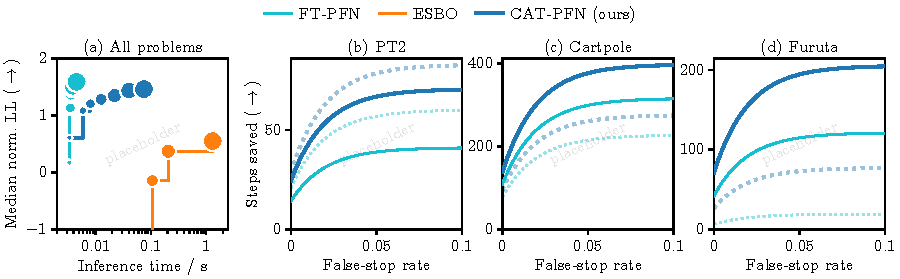
\includegraphics{figures/fig3.pdf}
  \caption{Prediction. (a) Median normalized log-likelihood against inference time (ESBO: its
    GP predictor), one
    marker per context size $N\in\{0,2,\dots,64\}$ on the Pareto front (marker size grows
    with $N$). (b--d) Steps saved on crashing trials against the false-stop rate; solid
    $N=64$, dotted $N=0$.}
  \label{fig:prediction}
\end{figure}

\begin{figure}[t]
  \centering
  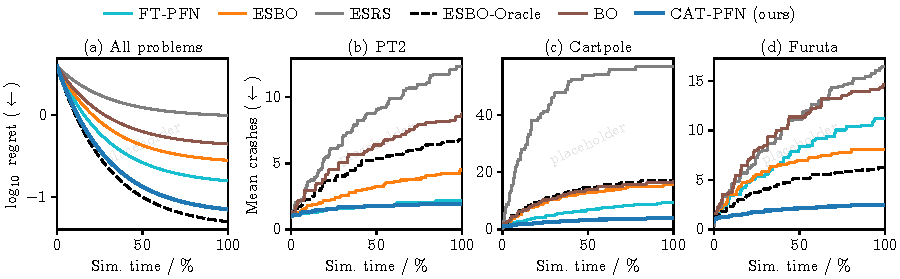
\includegraphics{figures/fig4.pdf}
  \caption{Simulation. (a) $\log_{10}$ regret over the simulated time budget, median
    over instances, mean over problems. (b--d) Mean number of crashed trials.}
  \label{fig:simulation}
\end{figure}

\begin{figure}[t]
  \centering
  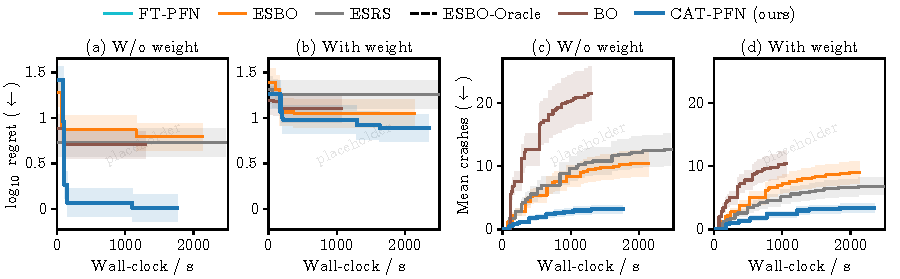
\includegraphics{figures/fig5.pdf}
  \caption{Hardware. (a, b) $\log_{10}$ regret (median over five seeds) and (c, d) crashed
    trials (mean), shaded 25--75\,\% over seeds, against wall-clock time, without and with
    the additional weight.}
  \label{fig:hardware}
\end{figure}

\lipsum[2-4]

\end{document}
